% Template do artigo do projeto (Sistemas Inteligentes, UFABC 2026.Q3)
% Conversão para LaTeX do EINF_SI_2026Q3_templateArtigoProjeto.docm,
% que é o template LNCS da Springer. Usa a classe oficial llncs (v2.24).
%
% Compilar:  latexmk -pdf artigo.tex      (ou: pdflatex artigo.tex duas vezes)
%
\documentclass[runningheads]{llncs}
%
% Página A4 com a área de texto do LNCS (12,2 x 19,3 cm) centralizada,
% igual ao template Word (margens de 4,4 cm nas laterais e 5,2 cm em cima e embaixo).
\usepackage[a4paper,textwidth=12.2cm,textheight=19.3cm,centering]{geometry}
\usepackage[T1]{fontenc}
% O template Word usa Times New Roman. Comente a linha abaixo para usar a
% fonte padrão do LNCS em LaTeX (Computer Modern).
\usepackage{mathptmx}
\usepackage{courier} % monoespaçada (e-mail, código) em Courier, como no Word
%
\usepackage{booktabs}
\usepackage{tabularx}
\usepackage{graphicx}
% Pastas onde o \includegraphics procura as figuras (ex.: as geradas pelo projeto.py)
\graphicspath{{figuras/}{../resultados/}}
\usepackage{pgfplots}
\pgfplotsset{compat=1.18}
\usepackage{listings}
\usepackage{xcolor}
\usepackage{hyperref}
\hypersetup{hidelinks}
\urlstyle{rm}
%
% Trechos de código em Python (o enunciado pede partes do código no artigo).
% Uso: \begin{lstlisting}[caption={Leitura do dataset.}, label={cod:leitura}] ... \end{lstlisting}
\lstset{
  language=Python,
  basicstyle=\ttfamily\footnotesize,
  numbers=left, numberstyle=\tiny, numbersep=6pt,
  frame=tb, breaklines=true, columns=fullflexible,
  keepspaces=true, showstringspaces=false, upquote=true,
  literate={á}{{\'a}}1 {à}{{\`a}}1 {ã}{{\~a}}1 {â}{{\^a}}1 {é}{{\'e}}1 {ê}{{\^e}}1
           {í}{{\'i}}1 {ó}{{\'o}}1 {õ}{{\~o}}1 {ô}{{\^o}}1 {ú}{{\'u}}1 {ç}{{\c c}}1
           {Á}{{\'A}}1 {É}{{\'E}}1 {Í}{{\'I}}1 {Ó}{{\'O}}1 {Ú}{{\'U}}1 {Ç}{{\c C}}1
           {º}{{\textordmasculine}}1 {ª}{{\textordfeminine}}1,
}
\AtBeginDocument{\renewcommand{\thelstlisting}{\arabic{lstlisting}}} % Código 1, 2, 3...
%
% ORCID como no Word: entre colchetes, com hífen (a classe usa modo matemático,
% que transforma o hífen em sinal de menos).
\renewcommand\orcidID[1]{\unskip\textsuperscript{[#1]}}
%
% ---------------------------------------------------------------------------
% Para escrever em português, descomente o bloco abaixo. Ele troca os rótulos
% (Resumo, Palavras-chave, Tabela, Referências, Agradecimentos...) e ativa a
% hifenização em português. O template original está em inglês.
% ---------------------------------------------------------------------------
%\usepackage[brazilian]{babel}
%\addto\captionsbrazilian{%
%  \def\abstractname{Resumo.}%
%  \def\keywordname{{\bfseries Palavras-chave:}}%
%  \def\ackname{Agradecimentos.}%
%  \def\discintname{Declaração de interesses.}%
%  \def\figurename{Fig.}%
%  \def\tablename{Tabela}%
%  \def\lstlistingname{Código}%
%}
%\def\andname{e}\def\lastandname{\unskip{} e} % "A, B e C" na lista de autores
%
\begin{document}
%
\title{Contribution Title}
%
% Título abreviado para o cabeçalho das páginas ímpares
\titlerunning{Contribution Title (shortened if too long)}
%
\author{João Pedro de Souza Prado (RA 11202130110) \and
Rafael Costoya (RA 11202320453) \and
Gustavo Prado Quinello (RA 11202421059)}
%
% Autores abreviados para o cabeçalho das páginas pares
\authorrunning{J. P. S. Prado et al.}
%
\institute{Fundação Universidade Federal do ABC}
%
\maketitle
\setcounter{footnote}{0} % notas de rodapé do texto começam em 1
%
\begin{abstract}
The abstract should summarize the contents of the paper in short terms,
i.e. 15--250 words.

\keywords{First Keyword, Second Keyword, Third Keyword.}
\end{abstract}
%
\section{Introduction}
\subsection{A Subsection Sample}
Please note that the first paragraph of a section or subsection is not
indented. The first paragraphs that follows a table, figure, equation etc.
does not have an indent, either.

Subsequent paragraphs, however, are indented.

\subsubsection{Sample Heading (Third Level).} Only two levels of headings
should be numbered. Lower level headings remain unnumbered; they are
formatted as run-in headings.

\paragraph{Sample Heading (Forth Level).} The contribution should contain
no more than four levels of headings. The following Table~\ref{tab1} gives
a summary of all heading levels.

\begin{table}
\caption{Table captions should be placed above the tables.}\label{tab1}
\centering
\renewcommand{\arraystretch}{1.15}
% Largura total do texto, colunas na mesma proporção do Word (1/4, 1/2, 1/4)
\begin{tabularx}{\textwidth}{p{0.2\textwidth}Xp{0.215\textwidth}}
\toprule[1.5pt]
Heading level & Example & Font size and style\\
\midrule[0.75pt]
Title (centered) & {\Large\bfseries Lecture Notes} & 14 point, bold\\
1\textsuperscript{st}-level heading & {\large\bfseries 1 Introduction} & 12 point, bold\\
2\textsuperscript{nd}-level heading & {\bfseries 2.1 Printing Area} & 10 point, bold\\
3\textsuperscript{rd}-level heading & {\bfseries Run-in Heading in Bold.} Text follows & 10 point, bold\\
4\textsuperscript{th}-level heading & {\itshape Lowest Level Heading.} Text follows & 10 point, italic\\
\bottomrule[1.5pt]
\end{tabularx}
\end{table}

\noindent Displayed equations are centered and set on a separate line.
\begin{equation}
x + y = z
\end{equation}
Please try to avoid rasterized images for line-art diagrams and schemas.
Whenever possible, use vector graphics instead (see Fig.~\ref{fig1}).

\begin{figure}
\centering
% Gráfico de exemplo do template, refeito em vetor com pgfplots.
% Para uma imagem, use: 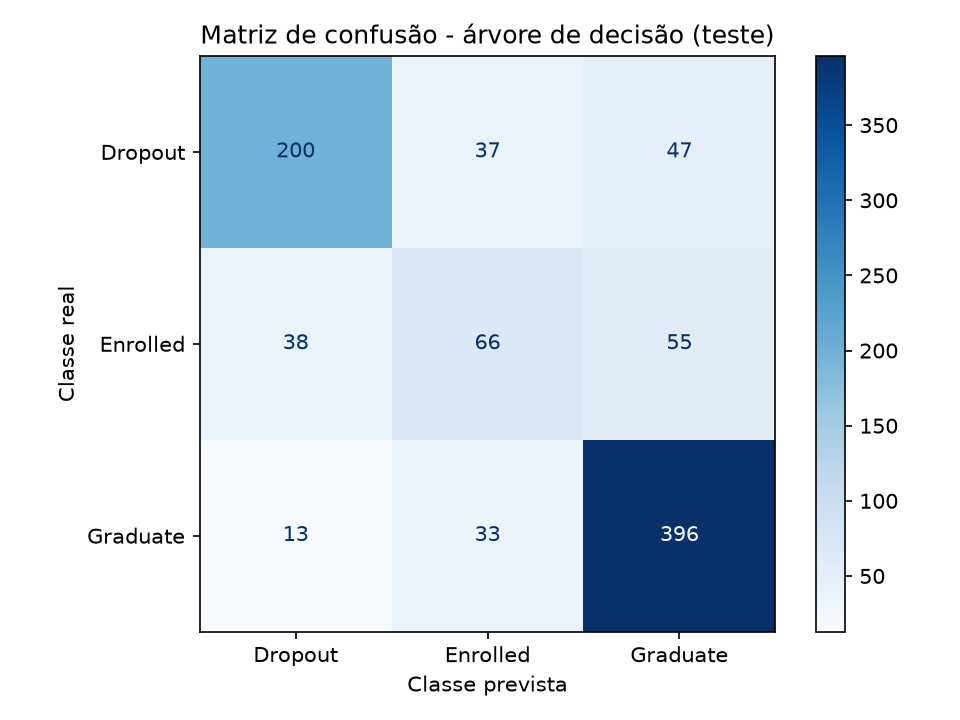
\includegraphics[width=\textwidth]{matriz_confusao.png}
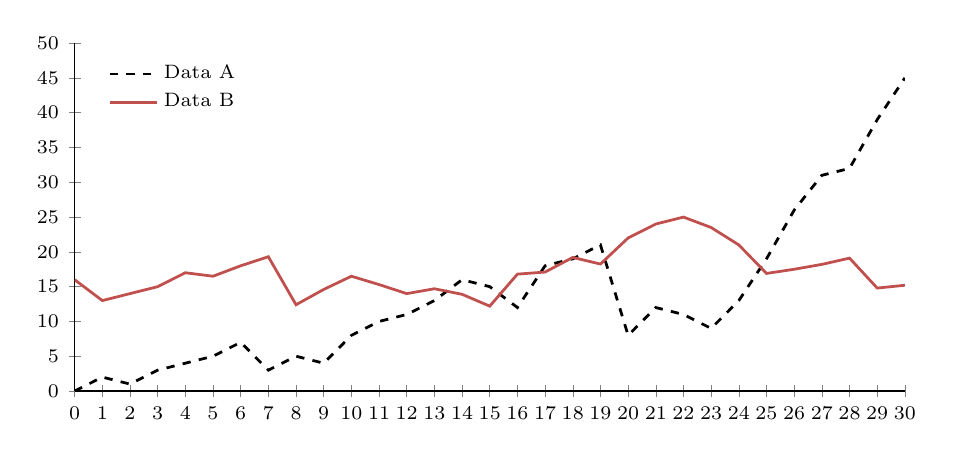
\begin{tikzpicture}
\begin{axis}[
  width=\textwidth, height=6cm,
  xmin=0, xmax=30, ymin=0, ymax=50,
  xtick={0,1,...,30}, ytick={0,5,...,50},
  axis x line=bottom, axis y line=left, axis line style={-},
  ticklabel style={font=\scriptsize},
  legend pos=north west, legend cell align=left,
  legend style={draw=none, font=\scriptsize, fill=none},
]
\addplot[black, dashed, line width=1pt] coordinates {
  (0,0) (1,2) (2,1) (3,3) (4,4) (5,5) (6,7) (7,3) (8,5) (9,4) (10,8)
  (11,10) (12,11) (13,13) (14,16) (15,15) (16,12) (17,18) (18,19) (19,21) (20,8)
  (21,12) (22,11) (23,9) (24,13) (25,19) (26,26) (27,31) (28,32) (29,39) (30,45)};
\addlegendentry{Data A}
\addplot[color={rgb,255:red,192;green,80;blue,77}, line width=1pt] coordinates {
  (0,16) (1,13) (2,14) (3,15) (4,17) (5,16.5) (6,18) (7,19.3) (8,12.4) (9,14.6) (10,16.5)
  (11,15.3) (12,14) (13,14.7) (14,13.9) (15,12.2) (16,16.8) (17,17.1) (18,19.2) (19,18.25) (20,22)
  (21,24) (22,25) (23,23.5) (24,21) (25,16.9) (26,17.5) (27,18.2) (28,19.1) (29,14.8) (30,15.2)};
\addlegendentry{Data B}
\end{axis}
\end{tikzpicture}
\caption{A figure caption is always placed below the illustration. Short
captions are centered, while long ones are justified. The macro button
chooses the correct format automatically.}\label{fig1}
\end{figure}

For citations of references, we prefer the use of square brackets and
consecutive numbers. Citations using labels or the author/year convention
are also acceptable. The following bibliography provides a sample reference
list with entries for journal articles~\cite{ref_article1}, an LNCS
chapter~\cite{ref_lncs1}, a book~\cite{ref_book1}, proceedings without
editors~\cite{ref_proc1}, as well as a URL~\cite{ref_url1}.

\section{Literature Review}

\section{Related works}

\section{Methodology}

\section{Results}

\section{Discussion}

\section{Conclusion}

\begin{credits}
\subsubsection{\ackname} A third level heading in 9-point font size at the
end of the paper is used for general acknowledgments, for example: This
study was funded by X (grant number Y).

\subsubsection{\discintname} It is now necessary to declare any competing
interests or to specifically state that the authors have no competing
interests. Please place the statement with a third level heading in 9-point
font size beneath the (optional) acknowledgments\footnote{If EquinOCS, our
proceedings submission system, is used, then the disclaimer can be provided
directly in the system.}, for example: The authors have no competing
interests to declare that are relevant to the content of this article. Or:
Author A has received research grants from Company W. Author B has received
a speaker honorarium from Company X and owns stock in Company Y. Author C is
a member of committee Z.
\end{credits}
%
% ---- Referências ----
% Lista manual, numerada na ordem em que aparece (como no template Word).
% Cite no texto com \cite{chave}. Exemplos no formato LNCS para o projeto:
%
% \bibitem{uci_dataset}
% Realinho, V., Vieira Martins, M., Machado, J., Baptista, L.: Predict
% Students' Dropout and Academic Success. UCI Machine Learning Repository
% (2021). \doi{10.24432/C5MC89}
%
% \bibitem{realinho2022}
% Realinho, V., Machado, J., Baptista, L., Martins, M.V.: Predicting Student
% Dropout and Academic Success. Data \textbf{7}(11), 146 (2022).
% \doi{10.3390/data7110146}
%
\begin{thebibliography}{8}
\bibitem{ref_article1}
Author, F.: Article title. Journal \textbf{2}(5), 99--110 (2016)

\bibitem{ref_lncs1}
Author, F., Author, S.: Title of a proceedings paper. In: Editor, F.,
Editor, S. (eds.) CONFERENCE 2016, LNCS, vol. 9999, pp. 1--13. Springer,
Heidelberg (2016)

\bibitem{ref_book1}
Author, F., Author, S., Author, T.: Book title. 2nd edn. Publisher,
Location (1999)

\bibitem{ref_proc1}
Author, F.: Contribution title. In: 9th International Proceedings on
Proceedings, pp. 1--2. Publisher, Location (2010)

\bibitem{ref_url1}
LNCS Homepage, \url{http://www.springer.com/lncs}, last accessed 2023/10/25
\end{thebibliography}
%
\end{document}
